\documentclass[a4paper,11pt]{article}
\usepackage{amsmath,amsthm,amsfonts,amssymb,amscd,amstext,vmargin,graphics,graphicx,tabularx,multicol} 
\usepackage[francais]{babel}
\usepackage[utf8]{inputenc}  
\usepackage[T1]{fontenc} 
\usepackage{pstricks-add,tikz,tkz-tab,variations}
\usepackage[autolanguage,np]{numprint} 
\usepackage{xlop}


\setmarginsrb{1.5cm}{0.5cm}{1cm}{0.5cm}{0cm}{0cm}{0cm}{0cm} %Gauche, haut, droite, haut
\newcounter{numexo}
\newcommand{\exo}[1]{\stepcounter{numexo}\noindent{\bf \underline{Exercice~\thenumexo}}}
\reversemarginpar

\opset{decimalsepsymbol={,}}
\newcounter{enumtabi}
\newcounter{enumtaba}
\newcommand{\q}{\stepcounter{enumtabi} \theenumtabi.  }
\newcommand{\qa}{\stepcounter{enumtaba} (\alph{enumtaba}) }
\newcommand{\initq}{\setcounter{enumtabi}{0}}
\newcommand{\initqa}{\setcounter{enumtaba}{0}}

\newcommand\hole[1]{$\bullet$}

\newcommand{\be}{\begin{enumerate}}
\newcommand{\ee}{\end{enumerate}}
\newcommand{\bi}{\begin{itemize}}
\newcommand{\ei}{\end{itemize}}
\newcommand{\bp}{\begin{pspicture*}}
\newcommand{\ep}{\end{pspicture*}}
\newcommand{\bt}{\begin{tabular}}
\newcommand{\et}{\end{tabular}}
\renewcommand{\tabularxcolumn}[1]{>{\centering}m{#1}} %(colonne m{} centrée, au lieu de p par défault) 
\newcommand{\tnl}{\tabularnewline}

\newcommand{\bmul}[1]{\begin{multicols}{#1}}
\newcommand{\emul}{\end{multicols}}

\newcommand{\trait}{\noindent \rule{\linewidth}{0.2mm}}
\newcommand{\hs}[1]{\hspace{#1}}
\newcommand{\vs}[1]{\vspace{#1}}

\newcommand{\N}{\mathbb{N}}
\newcommand{\Z}{\mathbb{Z}}
\newcommand{\R}{\mathbb{R}}
\newcommand{\C}{\mathbb{C}}
\newcommand{\Dcal}{\mathcal{D}}
\newcommand{\Ccal}{\mathcal{C}}
\newcommand{\mc}{\mathcal}

\newcommand{\vect}[1]{\overrightarrow{#1}}
\newcommand{\ds}{\displaystyle}
\newcommand{\eq}{\quad \Leftrightarrow \quad}
\newcommand{\vecti}{\vec{\imath}}
\newcommand{\vectj}{\vec{\jmath}}
\newcommand{\Oij}{(O;\vec{\imath}, \vec{\jmath})}
\newcommand{\OIJ}{(O;I,J)}




\newcommand{\reponse}[1][1]{%
\multido{}{#1}{\makebox[\linewidth]{\rule[0pt]{0pt}{20pt}\dotfill}
}}

\newcommand{\titre}[5] 
% #1: titre #2: haut gauche #3: bas gauche #4: haut droite #5: bas droite
{
\noindent #2 \hfill #4 \\
#3 \hfill #5

\vspace{-1.6cm}

\begin{center}\rule{6cm}{0.5mm}\end{center}
\vspace{0.2cm}
\begin{center}{\large{\textbf{#1}}}\end{center}
\begin{center}\rule{6cm}{0.5mm}\end{center}
}



\begin{document}
\pagestyle{empty}
\titre{Chapitre 5 : Les divisions}{}{}{}{}

\vspace*{1cm}

\begin{center}
{\Large \textbf{Niveau 1 :}}
\end{center}

\vspace*{1cm}

$\rightarrow$ \textbf{DIVISIONS EUCLIDIENNES : poser et savoir écrire une division euclidienne}\\

\vspace*{0.5cm}


\exo \\ Effectuer les divisions euclidiennes suivantes.\\

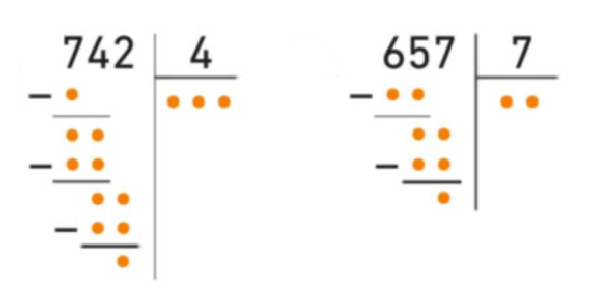
\includegraphics[scale=0.9]{de1.eps} \\



\exo \\ Compléter les bulles avec le bon vocabulaire.\\

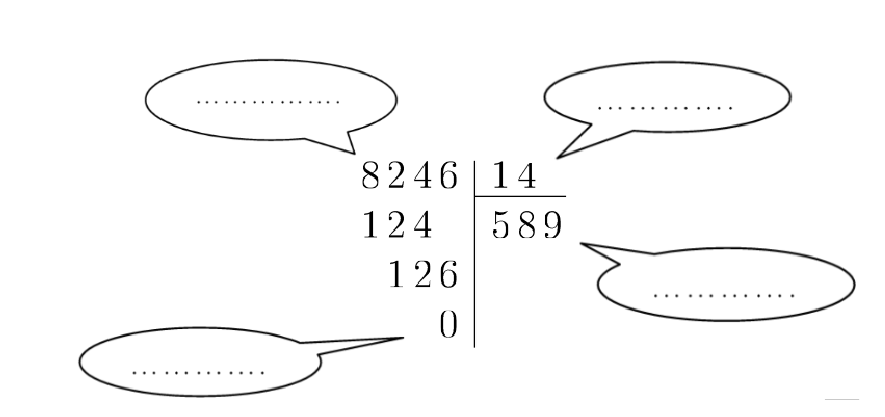
\includegraphics[scale=0.9]{diveucli1.eps} \\

\exo \\ Effectuer les divisions euclidiennes suivantes.\\

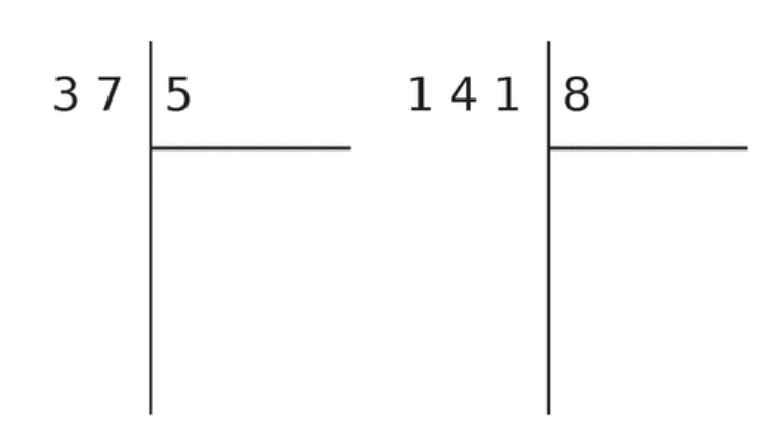
\includegraphics[scale=0.7]{de2.eps} \\




\vspace*{1cm}

$\rightarrow$ \textbf{DIVISIONS EUCLIDIENNES : multiples et critères de divisibilité}\\

\vspace*{0.5cm}

\exo \\ 
D'après l'égalité ci-dessous, compléter les phrases par le mot \textit{multiple} ou \textit{diviseur}.\\
\begin{center}
$12 \times 15 = 180$
\end{center}

\initqa
\qa 180 est un . . . . . . . . . . . . . de 12.\\

\qa 180 est un . . . . . . . . . . . . . de 15.\\

\qa 15 est un . . . . . . . . . . . . . de 180.\\

\qa 12 est un . . . . . . . . . . . . . de 180.\\


\exo \\ Compléter.\\

$21 = ( 7 \times .....)+ 0 $ donc 21 est . . . . . . . . . . . . . . par 7.\\
On dit aussi que 21 est un . . . . . . . . . . . . . . de 7 ou que 7 est un . . . . . . . . . . . . . . de 21.\\

\exo \\ Voici une liste de nombres : 240 ; 666 ; 745  ;  49  ; 136 ; 1 200.\\

\initqa \qa Quels sont les nombres de cette liste divisible par 2 ?\\
\reponse[2]\\


\qa Quels sont les nombres de cette liste divisible par 5 ?\\
\reponse[2]\\

\qa Peut-on en déduire les nombres  divisible par 10 ? Citer-les.\\
\reponse[2]\\

\exo \\ Voici une liste de nombres entiers.\\

\begin{center}
4 ; 10 ; 25 ; 27 ; 32 ; 50 ; 58 ; 65 ; 126.\\
\end{center}

Parmi ces nombres, lesquels sont :\\

\initqa \qa divisibles par 2 ? . . . . . . . . . . . . . . . . . . . . . . . . . . .\\

\qa des multiples de 5 ? . . . . . . . . . . . . . . . . . . . . . . . . . . .\\

\qa des diviseurs de 100 ? . . . . . . . . . . . . . . . . . . . . . . . . . . .\\


\exo \\ Voici une liste de nombres entiers.\\

\begin{center}
252 ; 351 ; 740 ; 1 548 ; 1 944.\\
\end{center}

Parmi ces nombres, lesquels sont :\\

\initqa \qa des multiples de 10 ? . . . . . . . . . . . . . . . . . . . . . . . . . . .\\

\qa divisibles par 2 ? . . . . . . . . . . . . . . . . . . . . . . . . . . .\\

\qa divisibles par 5 ? . . . . . . . . . . . . . . . . . . . . . . . . . . .\\


\vspace*{1cm}


$\rightarrow$ \textbf{DIVISIONS DÉCIMALE : calcul en colonne}\\

\textbf{Remarque :} Pour le niveau 1, ce serait intéressant de laisser l'élève compléter la division. Sur latex je n'arrive pas à tout cacher...
 
\vspace*{0.5cm}

\exo \\  Compléter la division suivante.\\



\opdiv[displayintermediary=nonzero,voperation=top,intermediarystyle.1.1=\hole,intermediarystyle.2.1=\hole,intermediarystyle.2.2=\hole,intermediarystyle.3.1=\hole,intermediarystyle.3.2=\hole,intermediarystyle.4.1=\hole,intermediarystyle.4.2=\hole,resultstyle=\hole]{117}{4}\\

Donc $117 \div 4 = . . . . . . .$\\

\exo \\  Compléter la division suivante.\\

\opdiv[displayintermediary=nonzero,voperation=top]{23}{5}\\
Donc $23 \div 5 = . . . . . . .$\\

\exo \\  Compléter la division suivante.\\

\opdiv[displayintermediary=nonzero,voperation=top]{27}{18}\\

Donc $27 \div 18 = . . . . . . .$\\


\exo \\  Compléter la division suivante.\\

\opdiv[displayintermediary=nonzero,voperation=top]{120}{25}\\

Donc $120 \div 25 = . . . . . . .$\\

\exo \\  Compléter la division suivante.\\

\opdiv[displayintermediary=nonzero,voperation=top]{1736}{64}\\

Donc $1736 \div 64 = . . . . . . .$\\


\vspace*{1cm}

$\rightarrow$ \textbf{DIVISIONS DÉCIMALES : calcul mental}\\

\vspace*{0.5cm}

\exo \\ Calculer mentalement.\\

\initqa \qa 70,6 $\div$ 10 = . . . . \\

\qa 51 $\div$ 10 = . . . . \\

\qa 1 352,69 $\div$ 10 = . . . . \\

\qa 5 240 $\div$ 10 = . . . . \\

\exo \\ Compléter les calculs suivants pour qu'ils soient justes.\\

\initqa \qa  5 427 $\div$ . . . .  = 54,27 \\

\qa  0,17 $\div$ . . . .  = 0,017 \\

\qa  . . . . $\div$ 100 = 4,8 \\

\qa  . . . . $\div$ 10  = 5,427 \\


\exo \\ Calculer mentalement.\\

\initqa \qa 12,6 $\div$ 2 = . . . . \\

\qa 93,3 $\div$ 3 = . . . . \\

\qa 5,5 $\div$ 5 = . . . . \\

\qa 12,4 $\div$ 4 = . . . . \\

\vspace*{1cm}

$\rightarrow$ \textbf{Problèmes sur les divisions euclidiennes et décimales}\\

\exo \\ Division euclidienne \\

Une bande de 6 enfants se partagent équitablement un sachet de 116 bonbons. Combien de bonbons recevra chaque enfant ?\\

Calculs :\\
\reponse[2]\\

Phrase réponse :\\
Chaque enfant recevra . . . bonbons et il en restera . . . \\

\exo \\ Division décimale \\
Mélanie a économisé tout son argent de poche cette année. Cela représente une somme de 474 euros. \\
Combien a-t-elle reçu à la fin de chaque mois?\\

Calculs :\\
\reponse[2]\\

Phrase réponse :\\
A la fin de chaque mois, Mélanie a reçu . . . . euros. \\

\exo \\ Division décimale \\
Pour chaque problème, écrire en ligne la ou les opération(s) à faire pour le résoudre. Ne faire aucun calcul.\\

\initqa \qa Patrick fait une randonnée de 2 jours de 56,3 km. Il a parcouru 9,6 km le premier matin.\\
Combien de kilomètre  lui reste-t-il à parcourir ?\\

Calculs :\\
\reponse[2]\\

\qa Caroline répartit 6,7 kg de miel dans 14 pots identiques.\\
Quel est le poids de chaque pot ?\\

Calculs :\\
\reponse[2]\\

\qa J'achète 11 pains au chocolat pour un total de 10,45 euros. \\
Combien coûte 3 pains au chocolat ?\\

Calculs :\\
\reponse[2]\\


	


\vspace*{0.5cm}


\vspace*{0.5cm}
\begin{center}
{\Large \textbf{Niveau 2 :}}
\end{center}

\vspace*{1cm}


$\rightarrow$ \textbf{DIVISIONS EUCLIDIENNES : poser et savoir écrire une division euclidienne}\\

\vspace*{0.5cm}


\exo \\ Effectuer les divisions euclidiennes suivantes et compléter les égalités qui leur correspondent.\\

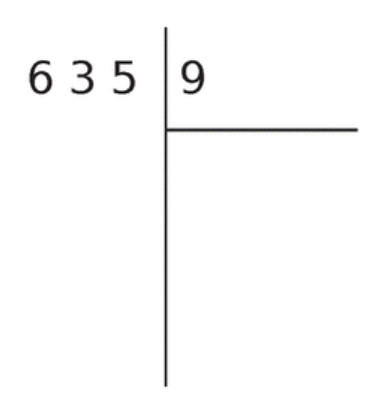
\includegraphics[scale=0.8]{de3b.eps} 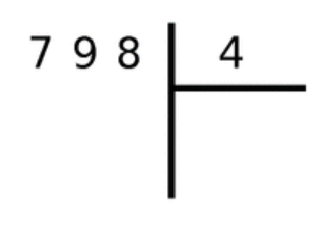
\includegraphics[scale=0.8]{de3a.eps} \\

$635 = (9 \times ....) + ....$ \hspace*{1.5cm} $798 = (4 \times ....) + ....$\\



\exo \\ Pour chacune des divisions euclidiennes ci-dessous, retrouver le dividende, le diviseur, le quotient et le reste.\\

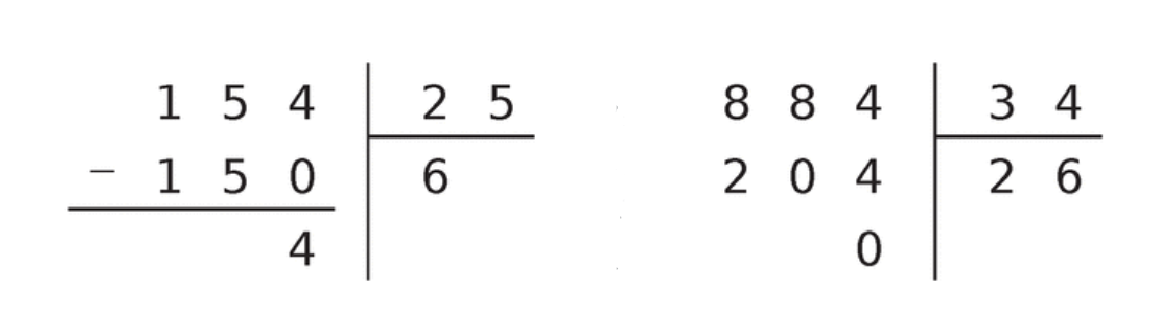
\includegraphics[scale=0.7]{de4.eps} \\

\bmul{2}

\noindent dividende : . . . . .\\
diviseur : . . . . .\\
quotient : . . . . .\\
reste : . . . . .\\

\columnbreak

\noindent dividende : . . . . .\\
diviseur : . . . . .\\
quotient : . . . . .\\
reste : . . . . .\\

\emul


\vspace*{1cm}

$\rightarrow$ \textbf{DIVISIONS EUCLIDIENNES : multiples et critères de divisibilité}\\

\vspace*{0.5cm}

\exo \\  Compléter les phrases suivantes par le mot \textit{multiple} ou \textit{diviseur}.\\

\initqa \qa 8 est un . . . . . . . . . . . . . de 32.\\

\qa 50 est un . . . . . . . . . . . . . de 5.\\

\qa 72 est un . . . . . . . . . . . . . de 9.\\

\qa 2 est un . . . . . . . . . . . . . de 48.\\

\exo \\ Écrire tous les multiples de 3 compris entre 14 et 32.\\

\noindent \reponse[3]\\


\exo \\  Compléter ce tableau (par \textit{oui} ou \textit{non} pour les 2 dernières lignes).\\

\begin{tabular}{|c|c|c|c|}
\hline 
Nombre & 507 & 829 & 5 310 \\ 
\hline 
Somme des chiffres & . . . . & . . . .  & . . . .  \\ 
\hline 
Le nombre est divisible par 3 & . . . .  & . . . .  & . . . .  \\ 
\hline 
Le nombre est divisible par 9 & . . . .  & . . . .  & . . . .  \\ 
\hline 
\end{tabular} 

\vspace*{0.3cm}

\exo \\ \exo \\ Voici une liste de nombres : 240 ; 666 ; 745  ;  49  ; 136 ; 1 200.\\

\initqa \qa Quels sont les nombres de cette liste divisible par 3 ?\\
\reponse[2]\\


\qa Quels sont les nombres de cette liste divisible par 9 ?\\
\reponse[2]\\

\qa Un nombre divisible par 3 est-il forcément divisible par 9 ?\\
\reponse[2]\\



\vspace*{1cm}


$\rightarrow$ \textbf{DIVISIONS DÉCIMALE : calcul en colonne}\\


 
\vspace*{0.5cm}

\exo \\ Poser la division décimale et donner le résultat approché au millième près.\\


\opdiv[displayintermediary=nonzero,voperation=top]{85}{6}\\

Donc $85 \div 6 \approx . . . . . . .$\\

\exo \\ Poser la division décimale et donner le résultat approché au millième près.\\


\opdiv[displayintermediary=nonzero,voperation=top]{12}{7}\\

Donc $12 \div 7 \approx . . . . . . .$\\

\exo \\ Poser la division décimale et donner le résultat approché au centième près.\\


\opdiv[displayintermediary=nonzero,voperation=top]{51}{21}\\

Donc $51 \div 21 \approx . . . . . . .$\\


\exo \\ Poser la division décimale et donner le résultat approché au centième près.\\


\opdiv[displayintermediary=nonzero,voperation=top]{10}{11}\\

Donc $10 \div 11 \approx . . . . . . .$\\


\vspace*{1cm}

$\rightarrow$ \textbf{DIVISIONS DÉCIMALES : calcul mental}\\

\vspace*{0.5cm}

\exo \\ Calculer mentalement.\\

\initqa \qa 589 $\div$ 100 = . . . . \\

\qa 14,59 $\div$ 100 = . . . . \\

\qa 11 581,3 $\div$ 100 = . . . . \\

\qa 5 970 $\div$ 100 = . . . . \\

\exo \\ Compléter les calculs suivants pour qu'ils soient justes.\\

\initqa \qa  17 532 $\div$ . . . .  = 17,532 \\

\qa 12,56 $\div$ . . . .  = 0,125 6 \\

\qa  . . . . $\div$ 1 000 = 18 \\

\qa  . . . . $\div$ 10  = 58,24 \\


\exo \\ Calculer mentalement.\\

\initqa \qa 12,6 $\div$ 3 = . . . . \\

\qa 120,6 $\div$ 6 = . . . . \\

\qa 2,4 $\div$ 3 = . . . . \\

\qa 0,63 $\div$ 9 = . . . . \\


\vspace*{1cm}

$\rightarrow$ \textbf{Problèmes sur les divisions euclidiennes et décimales}\\

\exo \\ Division euclidienne \\
La fleuriste dispose de 158 fleurs. Elle doit réaliser des bouquets de 7 fleurs chacun.\\

Combien de bouquets pourra-t-elle réaliser ?\\


Calculs :\\
\reponse[2]\\

Phrase réponse :\\
Elle pourra réaliser . . . de bouquets.\\

\exo Division décimale\\
Cédric a économisé tout son argent de poche cette année. Cela représente une somme de 494 euros. \\
Combien a-t-il reçu à la fin de chaque semaine?\\ 

Calculs :\\
\reponse[2]\\

Phrase réponse :\\
A la fin de chaque semaine, Cédric a reçu . . . . euros.\\

\vspace*{0.5cm}


\begin{center}
{\Large \textbf{Niveau 3 :}}
\end{center}

\vspace*{1cm}

$\rightarrow$ \textbf{DIVISIONS EUCLIDIENNES : poser et savoir écrire une division euclidienne}\\

\vspace*{0.5cm}


\exo \\ Effectuer les divisions euclidiennes suivantes et compléter les égalités qui leur correspondent.\\

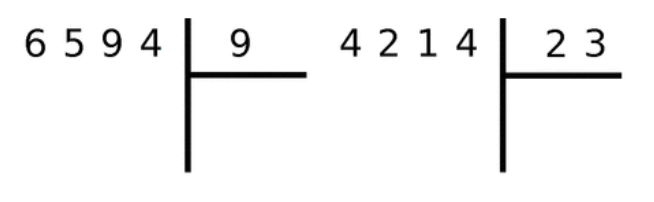
\includegraphics[scale=0.8]{de5.eps}\\

$6594 = (9 \times ....) + ....$ \hspace*{1.5cm} $4214 = (23 \times ....) + ....$\\


\exo \\ Écrire la division euclidienne correspondant à chacune de ces phrases.\\

\initqa 
\qa Le quotient de 745 par 7 est 106 et le reste est 3.\\
\begin{center}
 $....... = (...... \times ......) + ......$
\end{center}


\qa Le dividende est 78, le diviseur est 9, le quotient 8 et le reste 6.\\
\begin{center}
 $....... = (...... \times ......) + ......$
\end{center}

\exo \\ Pour chacune des divisions euclidiennes ci-dessous, écrire les égalités qui correspondent.\\


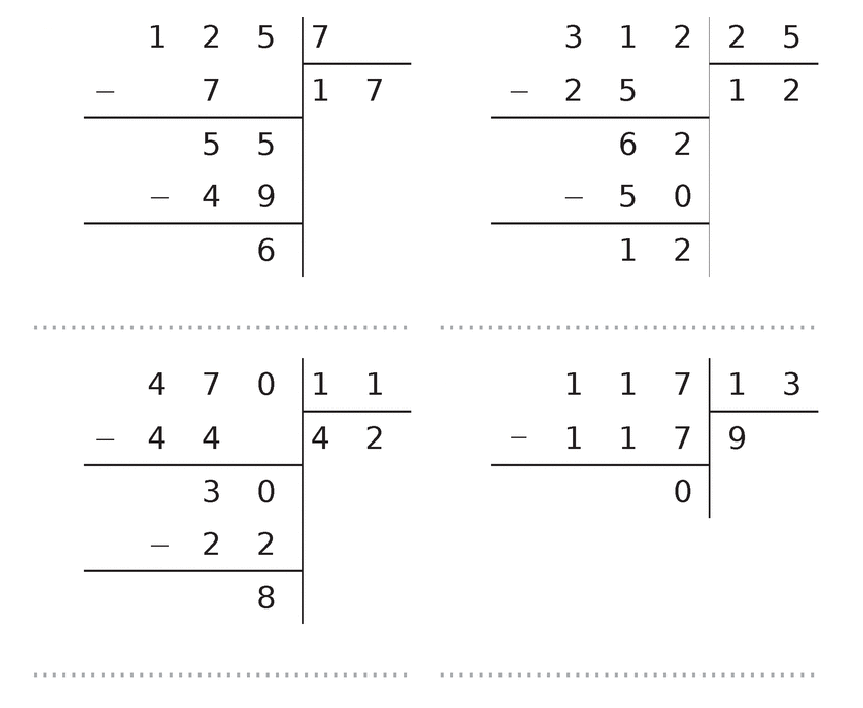
\includegraphics[scale=0.8]{de6.eps}\\


\exo \\ Compléter le tableau suivant.\\

\begin{tabular}{|c|c|c|}
\hline 
Division euclidienne de  & Quotient & Reste \\ 
\hline 
29 par 7  & . . . . & . . . . \\ 
\hline 
48 par 9 & . . . . & . . . . \\ 
\hline 
105 par 5 & . . . . & . . . . \\ 
\hline 
\end{tabular} 




\vspace*{1cm}

$\rightarrow$ \textbf{DIVISIONS EUCLIDIENNES : multiples et critères de divisibilité}\\

\vspace*{0.5cm}

\exo \\  Compléter les phrases suivantes par le mot \textit{multiple} ou \textit{diviseur}.\\

\initqa \qa 7 est un . . . . . . . . . . . . . de 42.\\

\qa 99 est un . . . . . . . . . . . . . de 11.\\

\qa 51 est un . . . . . . . . . . . . . de 17.\\

\qa 11 est un . . . . . . . . . . . . . de 33.\\

\exo \\ Écrire tous les multiples de 4 compris entre 38 et 52.\\

\noindent \reponse[3]\\




\exo \\ Dans chaque cas, dire si l'affirmation est vraie ou fausse.\\

\initqa \qa 125 est un multiple de 5.\\

\qa 7 est un multiple de 49.\\

\qa 12 est un diviseur de 36.\\

\qa 1 257 est divisible par 2.\\



\exo \\  Compléter ce tableau par \textit{oui} ou \textit{non}.\\

\begin{tabular}{|c|c|c|c|c|c|}
\hline 
est divisible par & 2 & 3 & 4 & 5 & 9 \\ 
\hline 
42 & . . . . & . . . . & . . . . & . . . . & . . . . \\ 
\hline 
100 & . . . . & . . . . & . . . . & . . . . & . . . . \\ 
\hline 
684 & . . . . & . . . . & . . . . & . . . . & . . . . \\ 
\hline 
\end{tabular} 

\vspace*{0.3cm}

\exo \\  Compléter ce tableau par \textit{oui} ou \textit{non}.\\

\begin{tabular}{|c|c|c|c|c|c|}
\hline 
est divisible par & 2 & 3 & 4 & 5 & 9 \\ 
\hline 
90 & . . . . & . . . . & . . . . & . . . . & . . . . \\ 
\hline 
825 & . . . . & . . . . & . . . . & . . . . & . . . . \\ 
\hline 
5 796 & . . . . & . . . . & . . . . & . . . . & . . . . \\ 
\hline 
\end{tabular} 

\vspace*{0.3cm}

\exo \\ \exo \\ Voici une liste de nombres : 240 ; 666 ; 744  ;  49  ; 136 ; 1 200.\\

\initqa \qa Quels sont les nombres de cette liste divisible par 4 ?\\
\reponse[2]\\



\vspace*{1cm}


$\rightarrow$ \textbf{DIVISIONS DÉCIMALE : calcul en colonne}\\


 
\vspace*{0.5cm}

\exo \\ Poser la division décimale et donner le résultat exact.\\


\opdiv[displayintermediary=nonzero,shiftdecimalsep=none,voperation=top]{7,6}{8}\\

Donc $7,6 \div 8 = . . . . . . .$\\

\exo \\ Poser la division décimale et donner le résultat exact.\\


\opdiv[displayintermediary=nonzero,shiftdecimalsep=none,voperation=top]{37,5}{5}\\

Donc $37,5 \div 5 = . . . . . . .$\\

\exo \\ Poser la division décimale et donner le résultat.\\


\opdiv[displayintermediary=nonzero,shiftdecimalsep=none,voperation=top]{28.8}{12}\\

Donc $28,8 \div 12 = . . . . . . .$\\


\vspace*{1cm}

$\rightarrow$ \textbf{DIVISIONS DÉCIMALES : calcul mental}\\

\vspace*{0.5cm}

\exo \\ Calculer mentalement.\\

\initqa \qa 8 975 $\div$ 1 000 = . . . . \\

\qa 317,54 $\div$ 1 000 = . . . . \\

\qa 5 780 $\div$ 1 000 = . . . . \\

\qa 123,6 $\div$ 1 000 = . . . . \\

\exo \\ Compléter les calculs suivants pour qu'ils soient justes.\\

\initqa \qa  514,78 $\div$ . . . .  = 5,147 8 \\

\qa  1 005,53 $\div$ . . . .  = 10,055 3 \\

\qa  . . . . $\div$ 100 = 3,70 \\

\qa  . . . . $\div$ 1 000  = 0,14 \\

\exo \\ Calculer mentalement.\\

\initqa \qa 48,6 $\div$ 9 = . . . . \\

\qa 4,2 $\div$ 3 = . . . . \\

\qa 0,01 $\div$ 2 = . . . . \\

\qa 12 $\div$ 60 = . . . . \\

\vspace*{0.5cm}

\vspace*{1cm}

$\rightarrow$ \textbf{Problèmes sur les divisions euclidiennes et décimales}\\

\exo \\ Division euclidienne \\
Pour le C.D.I. du collège, la documentaliste reçoit 370 livres qu'elle doit ranger sur des étagères. Elle ne peut transporter que 13 livres à chaque fois.\\
Combien de voyages minimum devra-t-elle faire ?  Et combien de livres transportera-t-elle au dernier voyage ?\\


Calculs :\\
\reponse[2]\\

Phrase réponse :\\
La documentaliste devra faire au minimum . . . . de voyages. Et au dernier voyage, elle portera . . . livres.\\



\exo \\ Division décimale\\
Paul a payé 44,66 euros pour 13 plants de tomate.\\
Quel est le prix d'un plant de tomate ?\\

Calculs :\\
\reponse[2]\\

Phrase réponse :\\
\\

\exo \\ Division décimale\\
Avec 24 kg de prunes, Chantal a fait 60 pots de confiture.\\
Quelle masse de prune contient chaque pot ?\\

Calculs :\\
\reponse[2]\\

Phrase réponse :\\
\reponse[2]\\

\vspace*{0.5cm}


\begin{center}
{\Large \textbf{Niveau 4:}}
\end{center}

\vspace*{1cm}

$\rightarrow$ \textbf{DIVISIONS EUCLIDIENNES : poser et savoir écrire une division euclidienne}\\

\vspace*{0.5cm}


\exo \\ Effectuer les divisions euclidiennes suivantes et compléter les égalités qui leur correspondent.\\

\textbf{Commentaire: Je n'arrive pas à écrire la division posée. Dans l'idéal il faudrait quelle le soit.}\\

1 941 $\div$ 27 \hspace*{1.5cm} 7 549 $\div$ 61\\



$1941 = (27 \times ....) + ....$ \hspace*{1.5cm} $7549 = (61 \times ....) + ....$\\




\exo \\ Compléter le tableau suivant.\\

\begin{tabular}{|c|c|c|}
\hline 
Division euclidienne de  & Quotient & Reste \\ 
\hline 
52 par 8  & . . . . & . . . . \\ 
\hline 
44 par 6 & . . . . & . . . . \\ 
\hline 
328 par 50 & . . . . & . . . . \\ 
\hline 
\end{tabular} 

\vspace*{0.5cm}


\vspace*{1cm}

$\rightarrow$ \textbf{DIVISIONS EUCLIDIENNES : multiples et critères de divisibilité}\\

\vspace*{0.5cm}


\exo \\ Écrire tous les multiples de 7 compris entre 47 et 85.\\

\noindent \reponse[3]\\




\exo \\ Dans chaque cas, dire si l'affirmation est vraie ou fausse.\\

\initqa \qa 425 est un multiple de 17.\\

\qa 32 est un diviseur de 1 552.\\

\qa 25 est un multiple de 175.\\


\qa 26 est divisible par 13 et par 1.\\


\exo \\ Parmi les nombres ci-dessous, citer ceux qui sont des diviseurs de 135.\\

\begin{center}
15 ; 95 ; 5 ; 100 ; 45 ; 4 et 9.
\end{center}

\noindent \reponse[2]\\

\exo \\ Parmi les nombres ci-dessous, citer ceux qui sont à la fois divisible par 3 et par 2.\\

\begin{center}
2 322 ; 42 ; 300 ; 1 022 ; 4 311 ; 24 et 65.
\end{center}

   \exo \\ Le code postal de Lilou est à la fois un multiple de 9 et divisible par 4.\\
   
   69 210 ; 83 420 ; 75 330 ; 59 940  ;  31 660.\\
   
   Quel est-il? . . . . . . . . . . . .\\
   
   
   
\vspace*{1cm}


$\rightarrow$ \textbf{DIVISIONS DÉCIMALE : calcul en colonne}\\


 
\vspace*{0.5cm}

\exo \\ Poser la division décimale et donner le résultat exact.\\


\opdiv[displayintermediary=nonzero,shiftdecimalsep=none,voperation=top]{42,9}{55}\\

Donc $42,9 \div 55 = . . . . . . .$\\

\exo \\ Poser la division décimale et donner le résultat exact.\\


\opdiv[displayintermediary=nonzero,shiftdecimalsep=none,voperation=top]{0,126}{9}\\

Donc $0,126 \div 9 = . . . . . . .$\\

\exo \\ Poser la division décimale et donner le résultat.\\


\opdiv[displayintermediary=nonzero,shiftdecimalsep=none,voperation=top]{5,49}{12}\\

Donc $5,49 \div 12 = . . . . . . .$\\
   
   
   \exo \\ Poser la division décimale et donner le résultat.\\


\opdiv[displayintermediary=nonzero,shiftdecimalsep=none,voperation=top]{2,013}{3}\\

Donc $2,013 \div 3 = . . . . . . .$\\

\vspace*{1cm}

$\rightarrow$ \textbf{DIVISIONS DÉCIMALES : calcul mental}\\

\vspace*{0.5cm}

\exo \\ Calculer mentalement.\\

\initqa \qa 51 035,1 $\div$ 10 000 = . . . . \\

\qa 102 008 $\div$ 10 000 = . . . . \\

\qa 9 815,301 $\div$ 10 000 = . . . . \\

\qa 127,4 $\div$ 10 000 = . . . . \\

\exo \\ Compléter les calculs suivants pour qu'ils soient justes.\\

\initqa \qa  157 005,3 $\div$ . . . .  = 1 570,053  \\

\qa  1,6 $\div$ . . . .  = 0,001 6 \\

\qa  . . . . $\div$ 100 = 0,12 \\

\qa  . . . . $\div$ 10 000 = 0,006 54 \\

\exo \\ Calculer mentalement.\\

\initqa \qa 10,2 $\div$ . . . . = 5,1 \\

\qa 6,15 $\div$ . . . . =  2,05 \\

\qa . . . . $\div$ 4 = 8,2 \\

\qa . . . .  $\div$ 9 = 1,01 \\

\vspace*{0.5cm}

\vspace*{1cm}

$\rightarrow$ \textbf{Problèmes sur les divisions euclidiennes et décimales}\\

\exo \\ Division euclidienne \\
Sur une planète, où poussent des fleurs immenses, un amoureux en cueille une dont la corolle a  258 839 pétales.
Il commence à l'effeuiller et il dit "Elle m'aime" en enlevant le premier pétale,"un peu" en enlevant le second, "beaucoup" en enlevant le troisième, puis "passionnément", "à la folie", "pas du tout". Et il recommence: "Elle m'aime", "un peu", "beaucoup"...\\

Quel mot va-t-il dire en effeuillant le dernier pétale?\\


Calculs :\\
\reponse[2]\\

Phrase réponse :\\
\\

\exo \\ Division euclidienne \\
Benjamin possède des billes. Il dit: "Je ne les ai pas comptées mais quand je les trie 5 par 5, il ne m'en reste pas. Quand je les trie 2 par 2, il m'en reste 1. Quand je les trie 6 par 6, il m'en reste 5. Je sais que j'en ai moins de 50."\\

 Combien de billes Benjamin possède t-il?\\

\exo \\ Division décimale\\
Une caisse contenant 30 objets identiques pèse 55,1 kg. Elle pèse à vide 1,1 kg.\\
Quelle est la masse en kg de chacun de ces objets ?\\

Calculs :\\
\reponse[2]\\

Phrase réponse :\\
Chaque objet pèse . . . kg.\\

\vspace*{0.5cm}
   
\begin{center}
{\Large \textbf{Niveau 5 :}}
\end{center}

\vspace*{1cm}

$\rightarrow$ \textbf{DIVISIONS EUCLIDIENNES : poser et savoir écrire une division euclidienne}\\

\vspace*{0.5cm}


\exo \\ Effectuer les divisions euclidiennes suivantes et compléter les égalités qui leur correspondent.\\

\textbf{Commentaire: Je n'arrive pas à écrire la division posée. Dans l'idéal il faudrait quelle le soit.}\\

7 045 $\div$ 103 \hspace*{1.5cm} 7 965 $\div$ 86\\



$7045 = (103 \times ....) + ....$ \hspace*{1.5cm} $7965 = (86 \times ....) + ....$\\




\exo \\ Compléter le tableau suivant.\\

\begin{tabular}{|c|c|c|c|}
\hline 
Dividende  & Diviseur & Quotient  & Reste\\ 
\hline 
789 & 14 & . . . . & . . . . \\ 
\hline 
. . . . & 13 & 9 & 7 \\ 
\hline 
14 502 & . . . . & 1 115 &7\\ 
\hline 
\end{tabular} 


\vspace*{1cm}

$\rightarrow$ \textbf{DIVISIONS EUCLIDIENNES : multiples et critères de divisibilité}\\

\vspace*{0.5cm}


\exo \\ Écrire tous les multiples de 9 compris entre 111 et 156.\\

\noindent \reponse[3]\\




\exo \\ Dans chaque cas, dire si l'affirmation est vraie ou fausse.\\

\initqa \qa 1 872 est divisible par 52 et par 117.\\

\qa 51 est un diviseur de 17.\\

\qa 24 est un multiple de 6 et un multiple de 8.\\


\qa 144 est à la fois un multiple de 36 et un diviseur de 6 156.\\


\exo \\ Donner le chiffre des unités manquant pour que le nombre soit divisible à la fois par 5 et par 3.\\

42? = . . . . . . . \hspace*{1cm} 52? = . . . . . . . \hspace*{1cm} 30? = . . . . . . . \hspace*{1cm} 12? = . . . . . . . \hspace*{1cm}\\


\exo \\ Quelle est la valeur du chiffre $\triangle$ pour que le nombre entier 3 52$\triangle$ soit divisible par 3 et par 5 ?\\
 Réponse : . . . . . . .\\
 
 
 \exo \\ Sur le ticket gagnant est inscrit un nombre qui est à la fois multiple de 4 et de 9.\\
 
 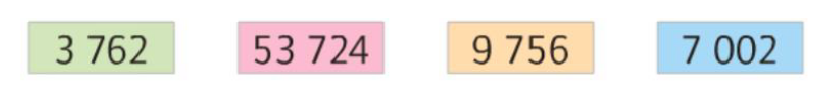
\includegraphics[scale=0.8]{critere1.eps} \\
 
 Quel est le ticket gagnant ? . . . . . . . . . .\\


\vspace*{0.5cm}

\vspace*{1cm}


$\rightarrow$ \textbf{DIVISIONS DÉCIMALE : calcul en colonne}\\


 
\vspace*{0.5cm}

\exo \\ Poser la division décimale et donner le résultat approché au millième près.\\


\opdiv[displayintermediary=nonzero,shiftdecimalsep=none,voperation=top]{123,8}{7}\\

Donc $123,8 \div 7 \approx . . . . . . .$\\

\exo \\ Poser la division décimale et donner le résultat approché au millième près.\\

\opdiv[displayintermediary=nonzero,shiftdecimalsep=none,voperation=top]{235,19}{11}\\

Donc $235,19 \div 11 \approx . . . . . . .$\\

\exo \\ Poser la division décimale et donner le résultat approché au centième près.\\

\opdiv[displayintermediary=nonzero,shiftdecimalsep=none,voperation=top]{0,145}{3}\\

Donc $0,145 \div 3 \approx . . . . . . .$\\

\exo \\ Poser la division décimale et donner le résultat approché au centième près.\\


\opdiv[displayintermediary=nonzero,shiftdecimalsep=none,voperation=top]{148,921}{12}\\

Donc $148,92 \div 12 \approx . . . . . . .$\\

\exo \\ Diviseur décimal. En vous appuyant sur l'exemple, transformer les divisions décimales pour que le diviseur ne soit plus un nombre décimal.\\

Exemple : 12,5 $\div$ 0,12 = 1 250 $\div$ 12\\

\initqa \qa 97,654 $\div$ 1,53 = . . . . . $\div$ . . . . .\\

\qa 285,8 $\div$ 0,6 = . . . . . $\div$ . . . . .\\

\qa 16,2  $\div$ 13,9 = . . . . . $\div$ . . . . .\\

\qa 125,61 $\div$ 0,025 = . . . . . $\div$ . . . . .\\



\vspace*{1cm}

$\rightarrow$ \textbf{DIVISIONS DÉCIMALES : calcul mental}\\

\vspace*{0.5cm}

\exo \\ Calculer mentalement.\\

\initqa \qa 0,6 $\div$ 100 = . . . . \\

\qa 8,91 $\div$ 1 000 = . . . . \\

\qa 0,78 $\div$ 100 = . . . . \\

\qa 0,04 $\div$ 10  = . . . . \\

\exo \\ Compléter les calculs suivants pour qu'ils soient justes.\\

\initqa \qa  4,5 $\div$ . . . .  = 0,000 45 \\

\qa  125,6 $\div$ . . . .  = 0,125 6 \\

\qa  . . . . $\div$ 1 000 = 0,3 \\

\qa  . . . . $\div$ 10 000  = 0,001 03 \\

\exo \\ Calculer mentalement.\\

\initqa \qa 8,25 $\div$ . . . . = 1,65 \\

\qa . . . . $\div$ 11 =  12,1\\

\qa . . . . $\div$ 5 = 3,08 \\

\qa 3,18  $\div$ . . . . = 1,06 \\

\vspace*{0.5cm}


\vspace*{1cm}

$\rightarrow$ \textbf{Problèmes sur les divisions euclidiennes et décimales}\\

\exo \\ Division euclidienne \\
Dans mon village, il y a 5 clubs :\\
- celui des Amis se réunit tous les 4 jours ;\\
- celui des Boulistes se réunit un jour sur trois ;\\
- celui des Chasseurs se réunit un jour sur deux ;\\
- celui des Danseurs se réunit tous les 5 jours ;\\
- celui des Enfants se réunit tous les 6 jours.\\

Aujourd'hui tous les clubs se sont réunis. Dans combien de jours se réuniront-ils à nouveau ?\\


Calculs :\\
\reponse[2]\\

Phrase réponse :\\
Les clubs se réuniront à nouveau dans . . . . jours.\\

\exo \\ Division euclidienne\\
Le centurion est fier de son armée. Pour le défilé à Rome, il demande à ses soldats de se ranger par lignes de cinq, mais il reste quatre soldats.\\
Il leur demande alors de se ranger par lignes de six, mais il reste cinq soldats.\\
Il leur demande de se ranger par lignes de huit, mais il reste sept soldats.\\

\noindent  Combien cette armée comporte-t-elle de soldats sachant qu'elle compte moins de deux-cents hommes ?\\

Calculs :\\
\reponse[2]\\

Phrase réponse :\\
Cette armée compte . . . . soldats.\\

\exo \\ Division euclidienne\\
La documentaliste d'un collège a posé une pile de 24 livres de 35 mm d'épaisseur chacun. A côté, elle a posé une autre pile de livre de 20 mm d'épaisseur chacun.Les deux piles ont la même hauteur.  \\

Combien y-a-t-il de livres dans la deuxième pile?\\

Calculs :\\
\reponse[2]\\

Phrase réponse :\\
\reponse[2]\\


\exo \\ Division décimale\\
Dans un champ de 8 000 $m^{2}$, l'agriculteur a eu besoin de 140 kg de graine de tournesol.\\

Quelle quantité de graine faut-il prévoir au $m^{2}$?\\

Calculs :\\
\reponse[2]\\

Phrase réponse :\\
\\


\exo \\ Division décimale\\
Dans un champ de 8 000 $m^{2}$, l'agriculteur a eu besoin de 140 kg de graine de tournesol.\\

Combien de graine faudrait-il pour un champ de 6 000 $m^{2}$?\\

Calculs :\\
\reponse[2]\\

Phrase réponse :\\
\reponse[2]\\
\vspace*{0.5cm}


\exo \\ Division décimale.\\
 Voici les tarifs pour un magazine mensuel :\\

- en kiosque, il coûte 99 euros pour un an (soit 12 magazines) ;\\

- en prenant un abonnement, les 12 numéros coûtent 63 euros et les 24 numéros coûtent 114 euros.\\


Quelle est la solution la plus avantageuse ?\\

Calculs :\\
\reponse[2]\\

Phrase réponse :\\
\reponse[2]\\




\end{document}
